One useful aspect of our first-order model~(\ref{e:first}) is that the solution to this differential equation is well known for a variety of input functions.  A particularly interesting input function is the \gls{step function} ($\mu(t)$) defined as
\begin{equation}
\label{e:step}
\mu(t)= \left\{ 
\begin{array}{cl}
0 & \, \mathrm{for}\, t < 0 \,\,\,\\
1 & \, \mathrm{for}\, t \geq 0
\end{array} \right.
.
\end{equation}
This function ($\mu(t)$) is also known as the \emph{unit} step function because the amplitude of the step is 1.0.
Figure~\ref{f:step} illustrates how the value of $\mu(t)$ is zero before $t=0$ and then instantaneously changes to unity.
\begin{figure}[hbt!]
\centering
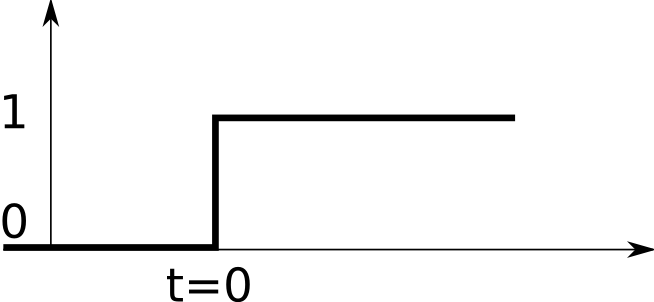
\includegraphics[width=\FigWidth\textwidth]{step.png}
\caption{Illustration of a step function $\mu(t)$.}
\label{f:step}
\end{figure}

Now consider our generic first-order model (\ref{e:first}) with a step input ($f(t)=A\mu(t)$) and an initial condition of zero ($y(0)=0$),
\begin{equation}
\label{e:firststepinput}
\frac{dy(t)}{dt} + \frac{1}{\tau}y(t) = A\mu(t).
\end{equation}
(You should notice that the input function ($f(t)$) is a step input with an amplitude of $A$.)
The \gls{step response} is the solution to this ordinary differential equation which is
\begin{equation}\label{e:stepresp}
y(t) = A\tau\left(1-e^{-t/\tau}\right)
\end{equation}
for $t>0$.  Notice that there are two key parameters of our model step response: the time constant ($\tau$) and the amplitude of the step input ($A$).

\begin{figure}[hbt]
\centering
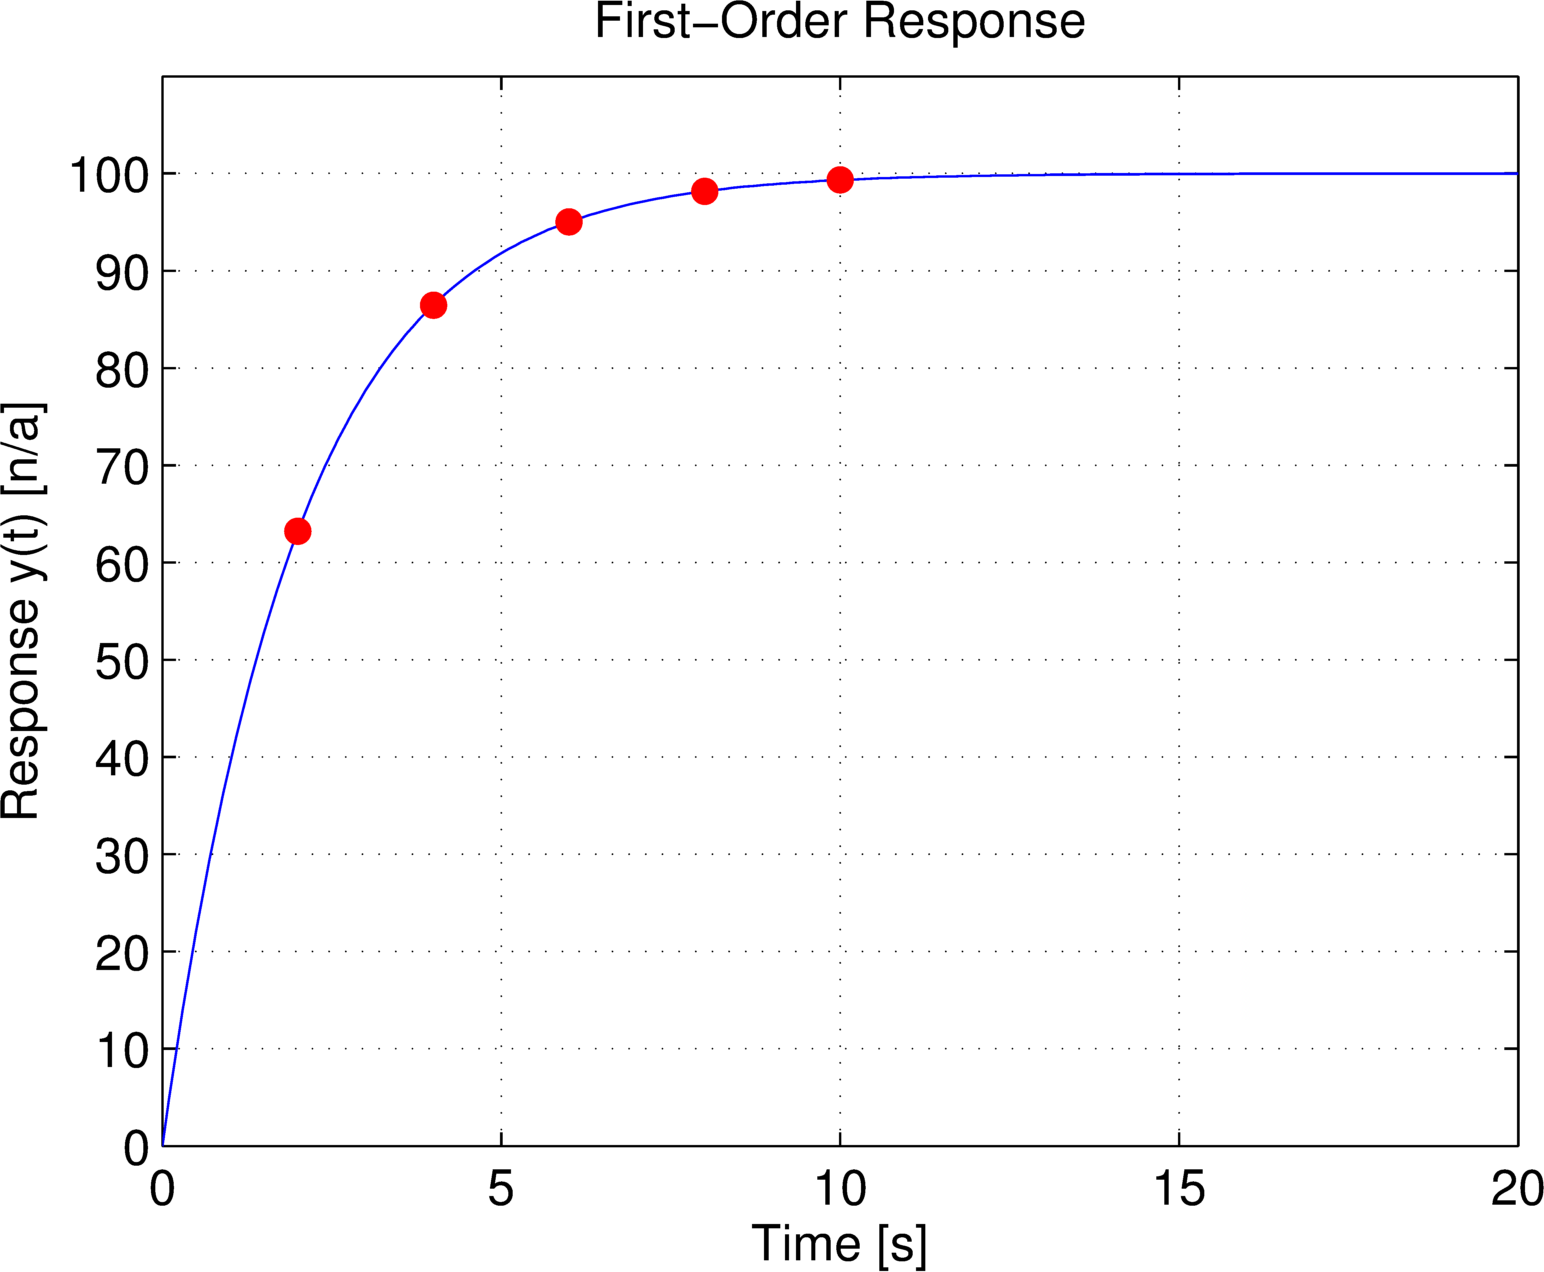
\includegraphics[width=\textwidth]{first_step.png}
\caption{Graph of the step response (\ref{e:stepresp}) with $\tau=\unit[2]{s}$ and $A=50$.  The red dot markers indicate the value of the solution at $t=[\tau,2\tau,3\tau,4\tau,5\tau]$. }
\label{f:firststep}
\end{figure}


\lstinputlisting[style=myMatStyle,
caption={Script for first-order response: first\_order\_response.m},
label={l:firstresp}]
{../code/first_order_response.m}


This solution (\ref{e:stepresp} is graphed in Figure~\ref{f:firststep} using the MATLAB script in Listing~\ref{l:firstresp}. This time response to a step input (or step response for short) has a characteristic shape as it rises and approaches the \gls{steady-state response} exponentially.  One important aspect of the response is that it approaches a new constant value, the steady-state response.  A simple way to find the steady state value is to set $\dot{y}(t)=0$ in (\ref{e:first}).  Since we are looking for the ``steady-state'' value we can anticipate that all rates of change (derivatives) will be zero.  Now the steady-state value ($y_{\mathrm{ss}}$) is 
\begin{equation}\label{e:ss}
y_{\mathrm{ss}} = \tau A.
\end{equation}

Another important characteristic of this model is that the response ($y(t)$) moves exponentially from the initial value to the steady state value.  This response is characterized by the the \gls{time constant} ($\tau$).  If we evaluate time response (\ref{e:stepresp}) at $t=\tau$ we find that
\[
y(t=\tau) = A \tau (0.632) = 0.632 (y_{\mathrm{ss}})
\]
which means that after one time constant has passed the response is 63.2\% of the way from the initial value to the steady state value.  Take a look at Figure~\ref{f:firststep} to make sure that we did the math correctly!
